\documentclass{beamer}
\usefonttheme{serif}
\usepackage{graphicx}
\usepackage{xcolor}
\usepackage{colortbl}
\usepackage{multirow,tabularx}
\usepackage{tikz}
\usepackage{hyperref}
\usepackage{physics}
\usepackage{siunitx}
\usepackage{amsthm}
\usepackage{amsmath}
\usepackage{caption}
\setlength{\belowcaptionskip}{-10pt}
\definecolor{blue}{rgb}{0.023, 0.113, 0.609}
\setbeamercolor{frametitle}{fg=blue}
\setbeamercolor{title}{fg=blue}
\setbeamercolor{structure}{fg=blue}
\setbeamertemplate{navigation symbols}{}
\title{Mathematical Foundations of Time Series Classification}
\subtitle{Wigner Summer Camp \\ Data and Compute Intensive Sciences Research Group}
\author{Bal\'azs, Paszk\'al, Vince, Levente, Antal \\ \'{E}va, Hajni}
\date{7--11 July 2025}

\hypersetup{
    colorlinks=true,
    linkcolor=blue,
    filecolor=magenta,      
    urlcolor=cyan,
    pdftitle={Overleaf Example},
    pdfpagemode=FullScreen,
    }

% Redefine footline to show only the slide number on the bottom left in blue
\setbeamertemplate{footline}
{
  \leavevmode%
  \hbox{%
  \begin{beamercolorbox}[wd=.1\paperwidth,ht=2.25ex,dp=1ex,left]{page number in head/foot}%
    \hspace{1em} \textcolor{blue}{\insertframenumber}%
  \end{beamercolorbox}}%Wigner Summer Camp

  \vskip0pt%
}

\begin{document}

\begin{frame}
  \titlepage
  \begin{columns}
    \centering
    \column{0.3\textwidth}
    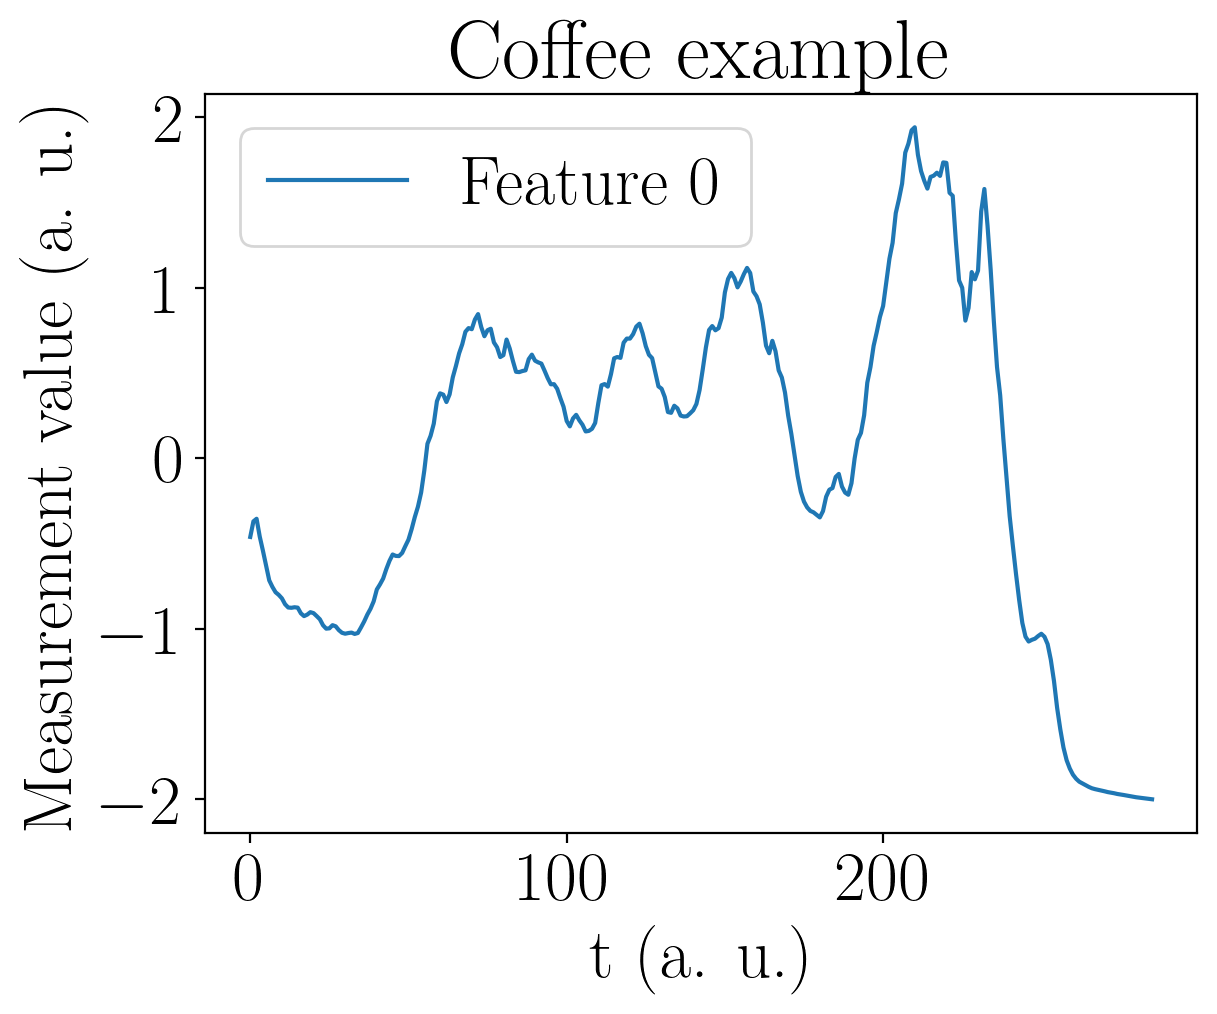
\includegraphics[width=0.7\textwidth]{../img/Coffee_example.png}
    \column{0.3\textwidth}
    \centering
    
\includegraphics[width=0.8\textwidth]{../img/logo.png}
    \column{0.3\textwidth}
          \begin{tabular}{|c|c|}
        \hline
          12 & 3 \\ \hline
          2 &  13 \\ \hline
      \end{tabular}
    \centering
  \end{columns}
\end{frame}

\begin{frame}{What is a Time Series?}
  A \textbf{time series} is a sequence of observations indexed by time.
  \\[1em]
  Examples include:
  \begin{itemize}
    \item Daily temperature readings
    \item Stock prices over time
    \item Sensor outputs in experiments
  \end{itemize}
  \begin{figure}[h]
    \centering
    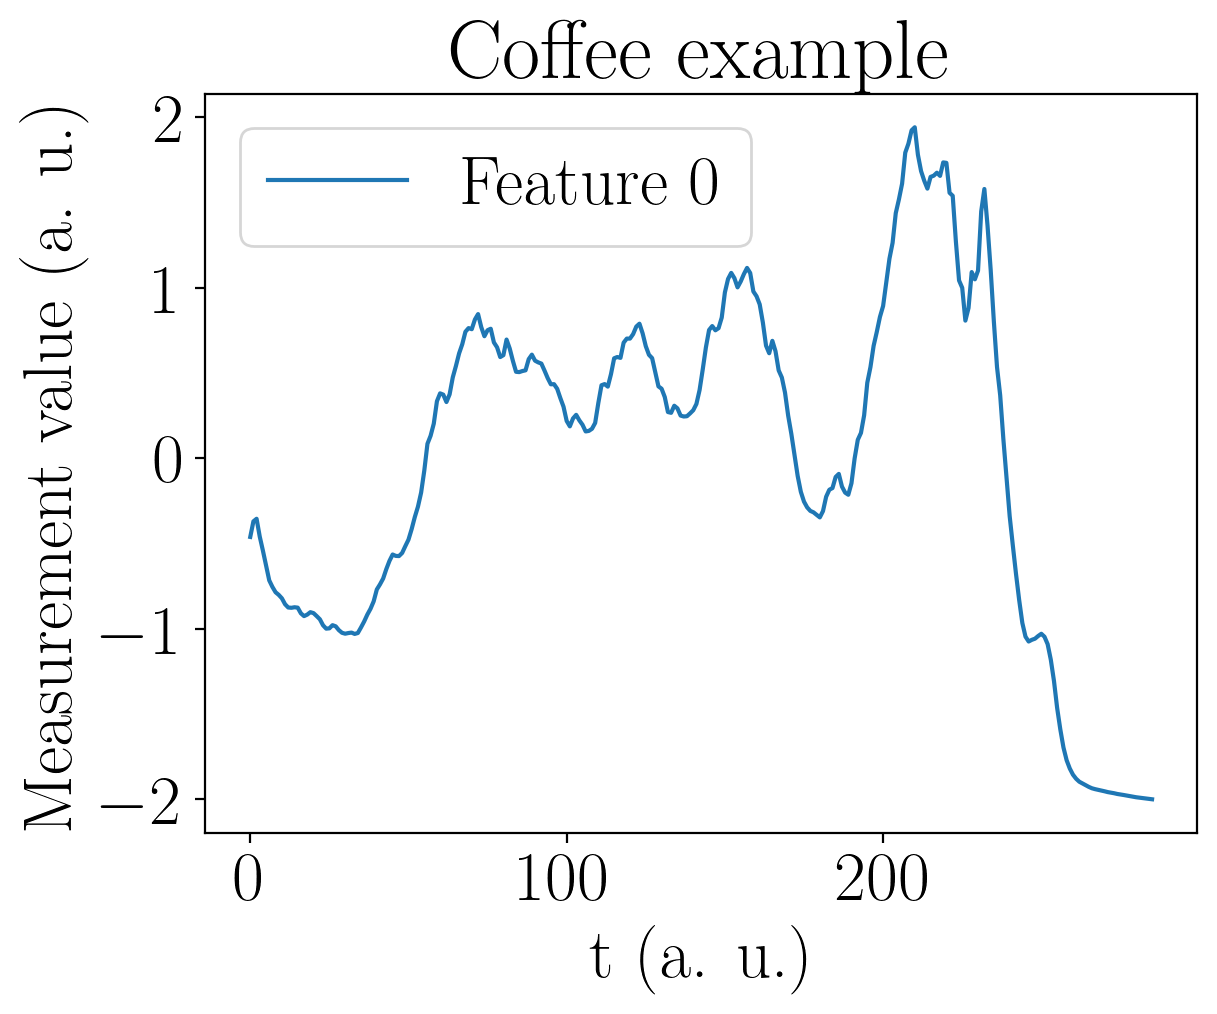
\includegraphics[width=0.5\textwidth]{../img/Coffee_example.png}
    \caption{Example of a univariate time series -- Coffee\cite{CoffeeDataset1996}.}
  \end{figure}
\end{frame}

\begin{frame}{What is Time Series Classification?}
  \textbf{Time Series Classification} (TSC) is the task of assigning a label to an entire time series.
  \\[1em]
  \textbf{Goal:} Learn a function \( f: \text{Series} \rightarrow \text{Class} \).
  \\[1em]
  \textbf{Applications:}
  \begin{itemize}
    \item Activity recognition (e.g., walking vs. running).
    \item Fault detection in engines.
    \item Medical diagnosis based on EEG/ECG.
  \end{itemize}
\end{frame}

\begin{frame}{(Common) Methods for TSC}
  \textbf{1. K-Nearest Neighbors (KNN)}:
  \begin{itemize}
    \item Classifies based on similarity.
  \end{itemize}
  \textbf{2. Neural Networks}:
  \begin{itemize}
    \item CNNs learn local patterns
    \item RNNs capture temporal dependencies.
  \end{itemize}
  \textbf{+1. ALT (Adaptive Law-Based Transformation)}\cite{kurbucz2025adaptive, halmos2025alt}:
  \begin{itemize}
    \item Transforms data into a linearly separable space.
    \item Transparent and interpretable.
  \end{itemize}
\end{frame}

\begin{frame}{The Confusion Matrix}
  \begin{table}[h]
    \centering
    \begin{tabular}{|c|c|c|}
      \hline
      & \textbf{Predicted: +} & \textbf{Predicted: -} \\
      \hline
      \textbf{Actual: +} & True Positive (TP) & False Negative (FN) \\
      \hline
      \textbf{Actual: -} & False Positive (FP) & True Negative (TN) \\
      \hline
    \end{tabular}
    \caption{Confusion Matrix}
  \end{table}
  \vspace{0.5em}
  \textbf{TP}: correctly predicted positive case. \\
  \textbf{TN}: correctly predicted negative case. \\
  \textbf{FP}: incorrectly predicted positive case. \\
  \textbf{FN}: missed positive case.
  \begin{table}[|c|c|]
      \centering
      \begin{tabular}{|c|c|}
        \hline
          12 & 3 \\ \hline
          2 &  13 \\ \hline
      \end{tabular}
      \caption{Example confusion matrix.}
      \label{tab:ex-conf-mat}
  \end{table}
\end{frame}

\begin{frame}{Evaluating Classifier Performance 2}
  \textbf{Metric Definitions:}
  \begin{itemize}
    \item \textbf{Accuracy}: Proportion of all correct predictions.
    \item \textbf{Precision}: \( \text{TP} / (\text{TP} + \text{FP}) \): Fraction of predicted positives that are true positives.
    \item \textbf{Recall (Sensitivity)}: \( \text{TP} / (\text{TP} + \text{FN}) \): Fraction of actual positives that are correctly identified.
    \item \textbf{F1-score}: Harmonic mean of precision and recall.
  \end{itemize}
  \vspace{1em}
  \textbf{Important Notes:}
  \begin{itemize}
    \item High accuracy can be misleading in imbalanced datasets.
    \item If the model predicts only the majority class, accuracy might still be high, but recall or precision will be low.
    \item F1-score helps balance precision and recall in such cases.
  \end{itemize}
\end{frame}

\begin{frame}{Example Calculation}
  \textbf{Confusion Matrix:}
  \begin{table}[h]
    \centering
    \begin{tabular}{|c|c|c|}
      \hline
      & Predicted + & Predicted - \\
      \hline
      Actual + & 40 (TP) & 5 (FN) \\
      \hline
      Actual - & 10 (FP) & 50 (TN) \\
      \hline
    \end{tabular}
  \end{table}
  \textbf{Metrics:}
  \begin{itemize}
    \item Accuracy: \( \frac{40 + 50}{105} = 0.857 \).
    \item Precision: \( \frac{40}{40 + 10} = 0.8 \).
    \item Recall: \( \frac{40}{40 + 5} \approx 0.889 \).
    \item F1-score: \( 2 \cdot \frac{0.8 \cdot 0.889}{0.8 + 0.889} \approx 0.842 \).
  \end{itemize}
\end{frame}

\begin{frame}{Exercise: Confusion Matrix Practice}
  \textbf{Confusion Matrix:}
  \begin{table}[h]
    \centering
    \begin{tabular}{|c|c|c|}
      \hline
      & Predicted + & Predicted - \\
      \hline
      Actual + & 30 (TP) & 15 (FN) \\
      \hline
      Actual - & 5 (FP) & 60 (TN) \\
      \hline
    \end{tabular}
  \end{table}
  \vspace{0.5em}
  Calculate:
  \begin{itemize}
    \item Accuracy
    \item Precision
    \item Recall
    \item F1-score
  \end{itemize}
\end{frame}

\begin{frame}{Solution}
  \textbf{Metrics:}
  \begin{itemize}
    \item Accuracy: \( \frac{30 + 60}{110} = 0.818 \).
    \item Precision: \( \frac{30}{30 + 5} = 0.857 \).
    \item Recall: \( \frac{30}{30 + 15} = 0.667 \).
    \item F1-score: \( 2 \cdot \frac{0.857 \cdot 0.667}{0.857 + 0.667} \approx 0.75 \).
  \end{itemize}
\end{frame}

\begin{frame}{Case 1: Imbalanced Dataset}
  \textbf{Confusion Matrix:}
  \begin{table}[h]
    \centering
    \begin{tabular}{|c|c|c|}
      \hline
      & Predicted + & Predicted - \\
      \hline
      Actual + (Minority) & 5 (TP) & 5 (FN) \\
      \hline
      Actual - (Majority) & 10 (FP) & 180 (TN) \\
      \hline
    \end{tabular}
  \end{table}
  \textbf{Metrics:}
  \begin{itemize}
    \item Accuracy: \( \frac{5 + 180}{200} = 0.925 \).
    \item Precision: \( \frac{5}{5 + 10} \approx 0.333 \).
    \item Recall: \( \frac{5}{5 + 5} = 0.5 \).
    \item F1-score: \( 2 \cdot \frac{0.333 \cdot 0.5}{0.333 + 0.5} \approx 0.4 \).
  \end{itemize}
  \textit{\small{High accuracy hides poor minority class performance.}}
\end{frame}

\begin{frame}{Case 2: Predicting All as One Class}
  \textbf{Confusion Matrix:}
  \begin{table}[h]
    \centering
    \begin{tabular}{|c|c|c|}
      \hline
      & Predicted + & Predicted - \\
      \hline
      Actual + & 0 (TP) & 50 (FN) \\
      \hline
      Actual - & 0 (FP) & 150 (TN) \\
      \hline
    \end{tabular}
  \end{table}
  \textbf{Metrics:}
  \begin{itemize}
    \item Accuracy: \( \frac{150}{200} = 0.75 \).
    \item Precision: Undefined (\( \frac{0}{0} \)), often set to 0.
    \item Recall: \( 0 \).
    \item F1-score: \( 0 \).
  \end{itemize}
  \textit{\small{Classifier completely ignores positive class.}}
\end{frame}

\begin{frame}{Case 3: Both Imbalanced and All One Class}
  \textbf{Confusion Matrix:}
  \begin{table}[h]
    \centering
    \begin{tabular}{|c|c|c|}
      \hline
      & Predicted - & Predicted + \\
      \hline
      Actual + (10) & 0 (TP) & 10 (FN) \\
      \hline
      Actual - (990) & 0 (FP) & 990 (TN) \\
      \hline
    \end{tabular}
  \end{table}
  \textbf{Metrics:}
  \begin{itemize}
    \item Accuracy: \( \frac{990}{1000} = 0.99 \).
    \item Precision: Undefined (\( \frac{0}{0} \)), often set to 0.
    \item Recall: \( 0 \).
    \item F1-score: \( 0 \).
  \end{itemize}
  \textit{\small{Extremely misleading: near-perfect accuracy, but model fails completely on minority class.}}
\end{frame}


\begin{frame}{References}
\bibliographystyle{IEEEtran}
\bibliography{references}
\end{frame}

\end{document}
